\subsubsubsubsection{Direction}
\begin{figure}[h]
\centering
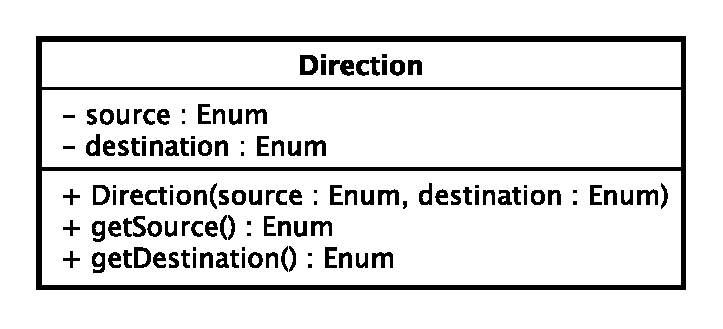
\includegraphics[scale=0.6,keepaspectratio]{images/solution/direction.eps}
\caption{App::Reactive::Direction}
\label{fig:sd-app-direction}
\end{figure}
\FloatBarrier
\begin{itemize}
  \item \textbf{Description} \\
    It represents the direction that a moving entity has while treading a
    street or a crossroads.
  \item \textbf{Attribute}
  \begin{itemize}
    \item \texttt{- source: Enum} \\
Direction from which an entity arrives. It may assume four possible
values: \{north, south, east, west\}.
    \item \texttt{- destination: Enum} \\
Direction the entity is going towards.  It also may assume four possible
values: \{north, south, east, west\}.
  \end{itemize}
\end{itemize}
